\documentclass{standalone}
\usepackage{tikz}
\usetikzlibrary{patterns, positioning}

\begin{document}
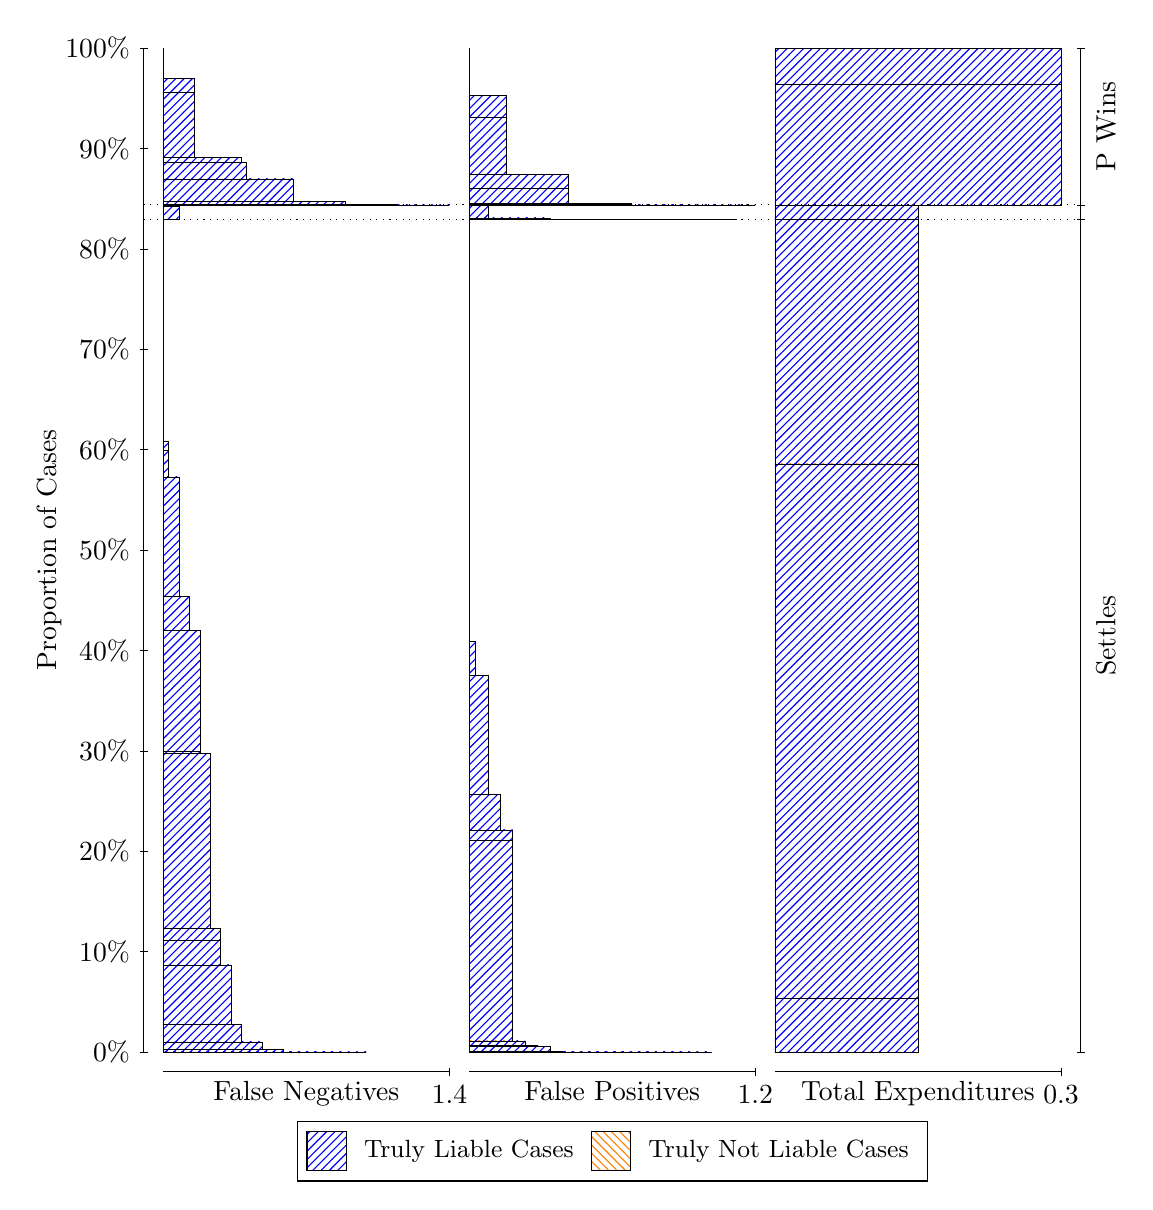
\begin{tikzpicture}
\draw[black, very thin] (1.5,1.75) -- (1.5,14.5);
\node[rotate=90, anchor=center] at (0.3, 8.125) {Proportion of Cases};
\draw[black, very thin] (1.45,1.75) -- (1.55,1.75);
\node[anchor=east] at (1.45, 1.75) {0\%};
\draw[black, very thin] (1.45,3.025) -- (1.55,3.025);
\node[anchor=east] at (1.45, 3.025) {10\%};
\draw[black, very thin] (1.45,4.3) -- (1.55,4.3);
\node[anchor=east] at (1.45, 4.3) {20\%};
\draw[black, very thin] (1.45,5.575) -- (1.55,5.575);
\node[anchor=east] at (1.45, 5.575) {30\%};
\draw[black, very thin] (1.45,6.85) -- (1.55,6.85);
\node[anchor=east] at (1.45, 6.85) {40\%};
\draw[black, very thin] (1.45,8.125) -- (1.55,8.125);
\node[anchor=east] at (1.45, 8.125) {50\%};
\draw[black, very thin] (1.45,9.4) -- (1.55,9.4);
\node[anchor=east] at (1.45, 9.4) {60\%};
\draw[black, very thin] (1.45,10.675) -- (1.55,10.675);
\node[anchor=east] at (1.45, 10.675) {70\%};
\draw[black, very thin] (1.45,11.95) -- (1.55,11.95);
\node[anchor=east] at (1.45, 11.95) {80\%};
\draw[black, very thin] (1.45,13.225) -- (1.55,13.225);
\node[anchor=east] at (1.45, 13.225) {90\%};
\draw[black, very thin] (1.45,14.5) -- (1.55,14.5);
\node[anchor=east] at (1.45, 14.5) {100\%};

\draw[black, very thin] (13.4,1.75) -- (13.4,14.5);
\draw[black, very thin] (13.35,1.75) -- (13.45,1.75);
\node[anchor=west] at (13.35, 1.75) {};
\draw[black, very thin] (13.35,12.321) -- (13.45,12.321);
\node[anchor=west] at (13.35, 12.321) {};
\draw[black, very thin] (13.35,12.509) -- (13.45,12.509);
\node[anchor=west] at (13.35, 12.509) {};
\draw[black, very thin] (13.35,14.5) -- (13.45,14.5);
\node[anchor=west] at (13.35, 14.5) {};

\draw[black, very thin, pattern color=blue, pattern=north east lines] (1.75,1.75) rectangle (4.3264,1.75);
\draw[black, very thin, pattern color=blue, pattern=north east lines] (1.75,1.75) rectangle (4.0621,1.75);
\draw[black, very thin, pattern color=blue, pattern=north east lines] (1.75,1.75) rectangle (3.7979,1.75);
\draw[black, very thin, pattern color=blue, pattern=north east lines] (1.75,1.75) rectangle (3.6658,1.75);
\draw[black, very thin, pattern color=blue, pattern=north east lines] (1.75,1.75) rectangle (3.5336,1.75);
\draw[black, very thin, pattern color=blue, pattern=north east lines] (1.75,1.75) rectangle (3.4015,1.75);
\draw[black, very thin, pattern color=blue, pattern=north east lines] (1.75,1.75) rectangle (3.2694,1.7839);
\draw[black, very thin, pattern color=blue, pattern=north east lines] (1.75,1.7839) rectangle (3.1373,1.7858);
\draw[black, very thin, pattern color=blue, pattern=north east lines] (1.75,1.7858) rectangle (3.0052,1.8771);
\draw[black, very thin, pattern color=blue, pattern=north east lines] (1.75,1.8771) rectangle (2.873,1.8782);
\draw[black, very thin, pattern color=blue, pattern=north east lines] (1.75,1.8782) rectangle (2.7409,2.1008);
\draw[black, very thin, pattern color=blue, pattern=north east lines] (1.75,2.1008) rectangle (2.6088,2.8556);
\draw[black, very thin, pattern color=blue, pattern=north east lines] (1.75,2.8556) rectangle (2.4767,3.1677);
\draw[black, very thin, pattern color=blue, pattern=north east lines] (1.75,3.1677) rectangle (2.4767,3.3222);
\draw[black, very thin, pattern color=blue, pattern=north east lines] (1.75,3.3222) rectangle (2.3445,5.5445);
\draw[black, very thin, pattern color=blue, pattern=north east lines] (1.75,5.5445) rectangle (2.2124,5.5723);
\draw[black, very thin, pattern color=blue, pattern=north east lines] (1.75,5.5723) rectangle (2.2124,7.106);
\draw[black, very thin, pattern color=blue, pattern=north east lines] (1.75,7.106) rectangle (2.0803,7.5355);
\draw[black, very thin, pattern color=blue, pattern=north east lines] (1.75,7.5355) rectangle (1.9482,9.0527);
\draw[black, very thin, pattern color=blue, pattern=north east lines] (1.75,9.0527) rectangle (1.8161,9.3922);
\draw[black, very thin, pattern color=blue, pattern=north east lines] (1.75,9.3922) rectangle (1.8161,9.5019);
\draw[black, very thin, pattern color=orange, pattern=north west lines] (1.75,9.5019) rectangle (1.75,9.5019);
\draw[black, very thin, pattern color=blue, pattern=north east lines] (1.75,9.5019) rectangle (1.75,12.321);
\draw[black, very thin, pattern color=blue, pattern=north east lines] (1.75,12.321) rectangle (1.9482,12.487);
\draw[black, very thin, pattern color=orange, pattern=north west lines] (1.75,12.487) rectangle (1.75,12.487);
\draw[black, very thin, pattern color=blue, pattern=north east lines] (1.75,12.487) rectangle (1.75,12.509);
\draw[black, very thin, pattern color=blue, pattern=north east lines] (1.75,12.509) rectangle (5.3833,12.509);
\draw[black, very thin, pattern color=blue, pattern=north east lines] (1.75,12.509) rectangle (4.7227,12.51);
\draw[black, very thin, pattern color=blue, pattern=north east lines] (1.75,12.51) rectangle (4.1282,12.51);
\draw[black, very thin, pattern color=blue, pattern=north east lines] (1.75,12.51) rectangle (4.0621,12.55);
\draw[black, very thin, pattern color=blue, pattern=north east lines] (1.75,12.55) rectangle (3.4676,12.55);
\draw[black, very thin, pattern color=blue, pattern=north east lines] (1.75,12.55) rectangle (3.4015,12.839);
\draw[black, very thin, pattern color=blue, pattern=north east lines] (1.75,12.839) rectangle (2.807,13.044);
\draw[black, very thin, pattern color=blue, pattern=north east lines] (1.75,13.044) rectangle (2.7409,13.116);
\draw[black, very thin, pattern color=blue, pattern=north east lines] (1.75,13.116) rectangle (2.1464,13.94);
\draw[black, very thin, pattern color=blue, pattern=north east lines] (1.75,13.94) rectangle (2.1464,14.112);
\draw[black, very thin, pattern color=blue, pattern=north east lines] (1.75,14.112) rectangle (2.0803,14.112);
\draw[black, very thin, pattern color=orange, pattern=north west lines] (1.75,14.112) rectangle (1.75,14.112);
\draw[black, very thin, pattern color=blue, pattern=north east lines] (1.75,14.112) rectangle (1.75,14.5);
\draw[black, very thin, pattern color=orange, pattern=north west lines] (5.6333,1.75) rectangle (8.7138,1.75);
\draw[black, very thin, pattern color=blue, pattern=north east lines] (5.6333,1.75) rectangle (8.7138,1.75);
\draw[black, very thin, pattern color=orange, pattern=north west lines] (5.6333,1.75) rectangle (8.3978,1.75);
\draw[black, very thin, pattern color=blue, pattern=north east lines] (5.6333,1.75) rectangle (8.3978,1.75);
\draw[black, very thin, pattern color=orange, pattern=north west lines] (5.6333,1.75) rectangle (8.0819,1.75);
\draw[black, very thin, pattern color=blue, pattern=north east lines] (5.6333,1.75) rectangle (8.0819,1.75);
\draw[black, very thin, pattern color=blue, pattern=north east lines] (5.6333,1.75) rectangle (7.9239,1.75);
\draw[black, very thin, pattern color=orange, pattern=north west lines] (5.6333,1.75) rectangle (7.7659,1.75);
\draw[black, very thin, pattern color=blue, pattern=north east lines] (5.6333,1.75) rectangle (7.7659,1.75);
\draw[black, very thin, pattern color=blue, pattern=north east lines] (5.6333,1.75) rectangle (7.608,1.75);
\draw[black, very thin, pattern color=orange, pattern=north west lines] (5.6333,1.75) rectangle (7.45,1.75);
\draw[black, very thin, pattern color=blue, pattern=north east lines] (5.6333,1.75) rectangle (7.45,1.75);
\draw[black, very thin, pattern color=blue, pattern=north east lines] (5.6333,1.75) rectangle (7.292,1.75);
\draw[black, very thin, pattern color=orange, pattern=north west lines] (5.6333,1.75) rectangle (7.1341,1.75);
\draw[black, very thin, pattern color=blue, pattern=north east lines] (5.6333,1.75) rectangle (7.1341,1.75);
\draw[black, very thin, pattern color=blue, pattern=north east lines] (5.6333,1.75) rectangle (6.9761,1.7503);
\draw[black, very thin, pattern color=orange, pattern=north west lines] (5.6333,1.7503) rectangle (6.8181,1.7503);
\draw[black, very thin, pattern color=blue, pattern=north east lines] (5.6333,1.7503) rectangle (6.8181,1.7546);
\draw[black, very thin, pattern color=blue, pattern=north east lines] (5.6333,1.7546) rectangle (6.6601,1.8184);
\draw[black, very thin, pattern color=orange, pattern=north west lines] (5.6333,1.8184) rectangle (6.5022,1.8184);
\draw[black, very thin, pattern color=blue, pattern=north east lines] (5.6333,1.8184) rectangle (6.5022,1.8184);
\draw[black, very thin, pattern color=blue, pattern=north east lines] (5.6333,1.8184) rectangle (6.5022,1.8329);
\draw[black, very thin, pattern color=blue, pattern=north east lines] (5.6333,1.8329) rectangle (6.3442,1.892);
\draw[black, very thin, pattern color=orange, pattern=north west lines] (5.6333,1.892) rectangle (6.1862,1.892);
\draw[black, very thin, pattern color=blue, pattern=north east lines] (5.6333,1.892) rectangle (6.1862,4.4338);
\draw[black, very thin, pattern color=blue, pattern=north east lines] (5.6333,4.4338) rectangle (6.1862,4.5692);
\draw[black, very thin, pattern color=blue, pattern=north east lines] (5.6333,4.5692) rectangle (6.0283,5.0184);
\draw[black, very thin, pattern color=blue, pattern=north east lines] (5.6333,5.0184) rectangle (5.8703,6.5356);
\draw[black, very thin, pattern color=blue, pattern=north east lines] (5.6333,6.5356) rectangle (5.7123,6.5356);
\draw[black, very thin, pattern color=blue, pattern=north east lines] (5.6333,6.5356) rectangle (5.7123,6.9651);
\draw[black, very thin, pattern color=blue, pattern=north east lines] (5.6333,6.9651) rectangle (5.6333,12.321);
\draw[black, very thin, pattern color=orange, pattern=north west lines] (5.6333,12.321) rectangle (9.0297,12.321);
\draw[black, very thin, pattern color=blue, pattern=north east lines] (5.6333,12.321) rectangle (9.0297,12.321);
\draw[black, very thin, pattern color=blue, pattern=north east lines] (5.6333,12.321) rectangle (8.2399,12.321);
\draw[black, very thin, pattern color=blue, pattern=north east lines] (5.6333,12.321) rectangle (7.45,12.321);
\draw[black, very thin, pattern color=blue, pattern=north east lines] (5.6333,12.321) rectangle (6.6601,12.344);
\draw[black, very thin, pattern color=blue, pattern=north east lines] (5.6333,12.344) rectangle (5.8703,12.509);
\draw[black, very thin, pattern color=orange, pattern=north west lines] (5.6333,12.509) rectangle (9.2667,12.509);
\draw[black, very thin, pattern color=blue, pattern=north east lines] (5.6333,12.509) rectangle (9.2667,12.509);
\draw[black, very thin, pattern color=orange, pattern=north west lines] (5.6333,12.509) rectangle (8.4768,12.509);
\draw[black, very thin, pattern color=blue, pattern=north east lines] (5.6333,12.509) rectangle (8.4768,12.509);
\draw[black, very thin, pattern color=blue, pattern=north east lines] (5.6333,12.509) rectangle (8.4768,12.509);
\draw[black, very thin, pattern color=orange, pattern=north west lines] (5.6333,12.509) rectangle (7.687,12.509);
\draw[black, very thin, pattern color=blue, pattern=north east lines] (5.6333,12.509) rectangle (7.687,12.517);
\draw[black, very thin, pattern color=blue, pattern=north east lines] (5.6333,12.517) rectangle (7.687,12.528);
\draw[black, very thin, pattern color=orange, pattern=north west lines] (5.6333,12.528) rectangle (6.9761,12.528);
\draw[black, very thin, pattern color=blue, pattern=north east lines] (5.6333,12.528) rectangle (6.9761,12.528);
\draw[black, very thin, pattern color=orange, pattern=north west lines] (5.6333,12.528) rectangle (6.8971,12.528);
\draw[black, very thin, pattern color=blue, pattern=north east lines] (5.6333,12.528) rectangle (6.8971,12.719);
\draw[black, very thin, pattern color=blue, pattern=north east lines] (5.6333,12.719) rectangle (6.8971,12.897);
\draw[black, very thin, pattern color=blue, pattern=north east lines] (5.6333,12.897) rectangle (6.1862,12.897);
\draw[black, very thin, pattern color=orange, pattern=north west lines] (5.6333,12.897) rectangle (6.1862,12.897);
\draw[black, very thin, pattern color=blue, pattern=north east lines] (5.6333,12.897) rectangle (6.1862,12.897);
\draw[black, very thin, pattern color=blue, pattern=north east lines] (5.6333,12.897) rectangle (6.1072,13.62);
\draw[black, very thin, pattern color=blue, pattern=north east lines] (5.6333,13.62) rectangle (6.1072,13.894);
\draw[black, very thin, pattern color=orange, pattern=north west lines] (5.6333,13.894) rectangle (5.6333,13.894);
\draw[black, very thin, pattern color=blue, pattern=north east lines] (5.6333,13.894) rectangle (5.6333,14.5);
\draw[black, very thin, pattern color=orange, pattern=north west lines] (9.5167,1.75) rectangle (11.333,1.75);
\draw[black, very thin, pattern color=blue, pattern=north east lines] (9.5167,1.75) rectangle (11.333,2.4377);
\draw[black, very thin, pattern color=orange, pattern=north west lines] (9.5167,2.4377) rectangle (11.333,2.4377);
\draw[black, very thin, pattern color=blue, pattern=north east lines] (9.5167,2.4377) rectangle (11.333,9.2176);
\draw[black, very thin, pattern color=orange, pattern=north west lines] (9.5167,9.2176) rectangle (11.333,9.2176);
\draw[black, very thin, pattern color=blue, pattern=north east lines] (9.5167,9.2176) rectangle (11.333,12.321);
\draw[black, very thin, pattern color=orange, pattern=north west lines] (9.5167,12.321) rectangle (11.333,12.321);
\draw[black, very thin, pattern color=blue, pattern=north east lines] (9.5167,12.321) rectangle (11.333,12.509);
\draw[black, very thin, pattern color=orange, pattern=north west lines] (9.5167,12.509) rectangle (13.15,12.509);
\draw[black, very thin, pattern color=blue, pattern=north east lines] (9.5167,12.509) rectangle (13.15,14.039);
\draw[black, very thin, pattern color=orange, pattern=north west lines] (9.5167,14.039) rectangle (13.15,14.039);
\draw[black, very thin, pattern color=blue, pattern=north east lines] (9.5167,14.039) rectangle (13.15,14.5);
\draw[black, dotted] (1.5,12.321) -- (13.4,12.321);
\draw[black, dotted] (1.5,12.509) -- (13.4,12.509);
\draw[black, very thin] (1.75,1.5) -- (5.3833,1.5);
\node[anchor=north] at (3.5667, 1.5) {False Negatives};
\draw[black, very thin] (5.3833,1.45) -- (5.3833,1.55);
\node[anchor=north] at (5.3833, 1.45) {1.4};

\draw[black, very thin] (5.6333,1.5) -- (9.2667,1.5);
\node[anchor=north] at (7.45, 1.5) {False Positives};
\draw[black, very thin] (9.2667,1.45) -- (9.2667,1.55);
\node[anchor=north] at (9.2667, 1.45) {1.2};

\draw[black, very thin] (9.5167,1.5) -- (13.15,1.5);
\node[anchor=north] at (11.333, 1.5) {Total Expenditures};
\draw[black, very thin] (13.15,1.45) -- (13.15,1.55);
\node[anchor=north] at (13.15, 1.45) {0.3};

\node[black, centered, rotate=90] at (13.72, 7.0355) {Settles};

\node[black, centered, rotate=90] at (13.72, 13.505) {P Wins};

\draw (7.449999999999999,1.5) node[draw=none] (baseCoordinate) {};
\begin{scope}[align=center]
        \matrix[scale=0.5, draw=black, below=0.5cm of baseCoordinate, nodes={draw}, column sep=0.1cm]{
            \node[rectangle, draw, minimum width=0.5cm, minimum height=0.5cm, pattern=north east lines, pattern color=blue] {}; &
            \node[draw=none, font=\small] (B) {Truly Liable Cases}; &
            \node[rectangle, draw, minimum width=0.5cm, minimum height=0.5cm, pattern=north west lines, pattern color=orange] {}; &
            \node[draw=none, font=\small] (B) {Truly Not Liable Cases}; \\
            };
\end{scope}

\end{tikzpicture}
\end{document}